\documentclass[article]{IEEEtran}
\usepackage[utf8]{inputenc}
\usepackage{graphicx}
\usepackage{cite}
\usepackage{url}

\title{Week 2. Assignment \\
\large UCCS CS 6000 Computer Science Research}

\author{Jose Luis Castanon Remy}
\date{September 2022}

\begin{document}

\maketitle




\section{Research direction}
During my last working experience, I always had the idea that our security systems were in place but not in the correct way. Similar to a wind power plant, the plant is placed in a windy area but if the back of the fan is not correctly placed facing the wind, the blades are not able to generate any movement and as a consequence, no electricity is being drawn from the wind.

Somehow our systems were there, we were able to log information from different sub-systems, but we were not focusing our efforts on the areas that needed more time (at a first glance there was a lot on our plates). For instance, we were not analyzing the collected data from logs and other systems. I always had the feeling that all the security systems in place were not able to give us the real "whole picture" of our security status. We had different tools giving us different metrics in different places. During my time there, my duties did not let me think about the critical problem behind all that "confusion". In addition to this, we were not able to map all the assets that needed protection. Most of those were newly discovered after we had our tools and myself analyze the architecture and the systems built within the company. 

I feel that companies should have a way to centralize metrics as well as compound a list of assets to be used in different security processes. One of the questions that come up is, What metrics need to be centralized? 

Related to this initial idea, comes up the following question, What metrics can show us the real "whole picture" of our security status? 

In order to get a proper understanding of the initial  direction, I should not be just mapping software but assessing software qualities that can give us a valuable metric pool to measure within the software. 

To address the issue, my advisor gave me a hint to research software (SW) maintenance and maintainability. SW maintenance/ maintainability can lead to specific aspects within SW that can lead to a better understanding of security issues, help detect areas with flaws, etc.

I have compiled the following list of papers:
\cite{alsolai2020systematic}, \cite{khezami2021systematic}, \cite{malhotra2016software}, \cite{malhotra2020systematic}, \cite{tian2021impact} and \cite{riaz2009systematic}.
Most of the notes are within the printed version of the 4 papers that I have chosen to read. I will be adding the keynotes to the bibliography.

\section{Reading}
From the list of papers that I have selected to read, 3 of them are related to software maintainability and one of those is related to software maintenance. Before getting to the analysis, I should be reading more about software maintenance. I feel that I need to research a little bit more in that direction.

Within the selected papers, published years in descending order are 2021 \cite{khezami2021systematic}, 2020 \cite{malhotra2020systematic}, \cite{alsolai2020systematic} and 2016 \cite{malhotra2016software}. I have read a survey paper about software maintenance from 2009, \cite{riaz2009systematic}, which I found to be very helpful in order to get myself older trends and perspectives.

The most cited paper, currently 55 citations, based on Google Scholar information, is related to software maintainability prediction \cite{alsolai2020systematic}. I think it is a highly cited paper because it contains very helpful components within its organization. It is the only paper that I have read that contains a good process review diagram. There is a data extraction analysis that is directly related to the research questions. I consider this is very helpful. It is introducing in a simple way the main ideas that the researchers have encountered during the literature review process. In general, I got the feeling that everything within this paper is helpful. There is nothing that I feel is useless in this paper. I have not had this "feeling" with the rest of the papers that I have read.

Related to the concepts that were introduced in class, This paper is able to answer all the Ws. The paper is correctly structured and there are relevant details that help me narrow some of my initial research questions.

The rest of the papers with lower citations, are either too focused on machine learning methods and prediction algorithms, which I do not feel are going to be helpful right now, or these papers contain useless/ non-structured information. Most of those fail to answer the "for whom" questions specifically to me.



\section{Topic map}
I have built the following topic maps. The first one is the map of the topics coming out from the papers that I have decided to read. These topics are repeated and color-ordered.

\begin{figure}[htp]
    \centering
    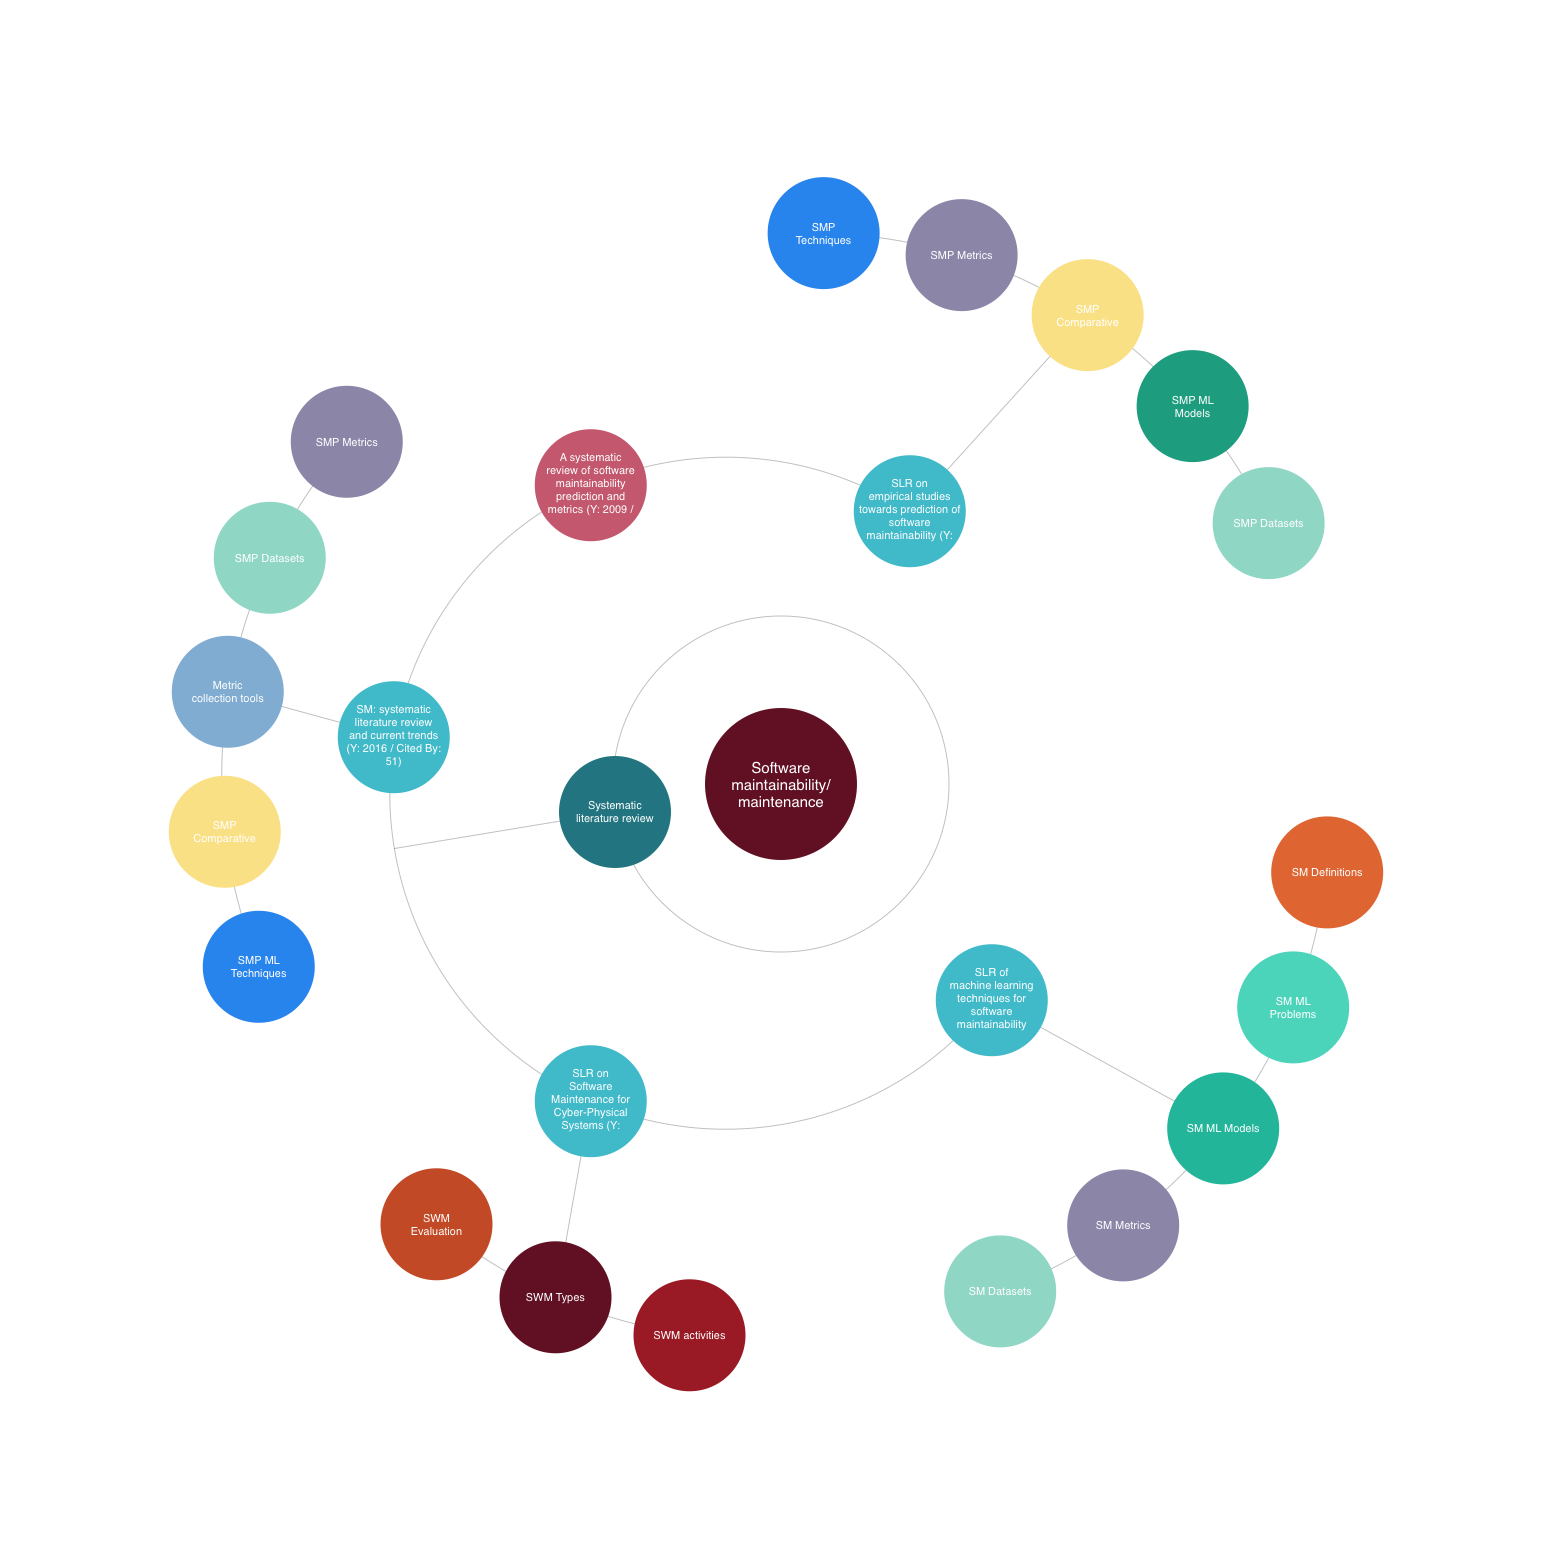
\includegraphics[width=8.5cm]{topics_per_paper.png}
    \caption{Topics per paper}
    \label{fig:topicspp}
\end{figure}

The second map is an organized map of the first one. It is organized by topic, software maintenance or maintainability, and the topics that came out from the previous topic map.

\begin{figure}[htp]
    \centering
    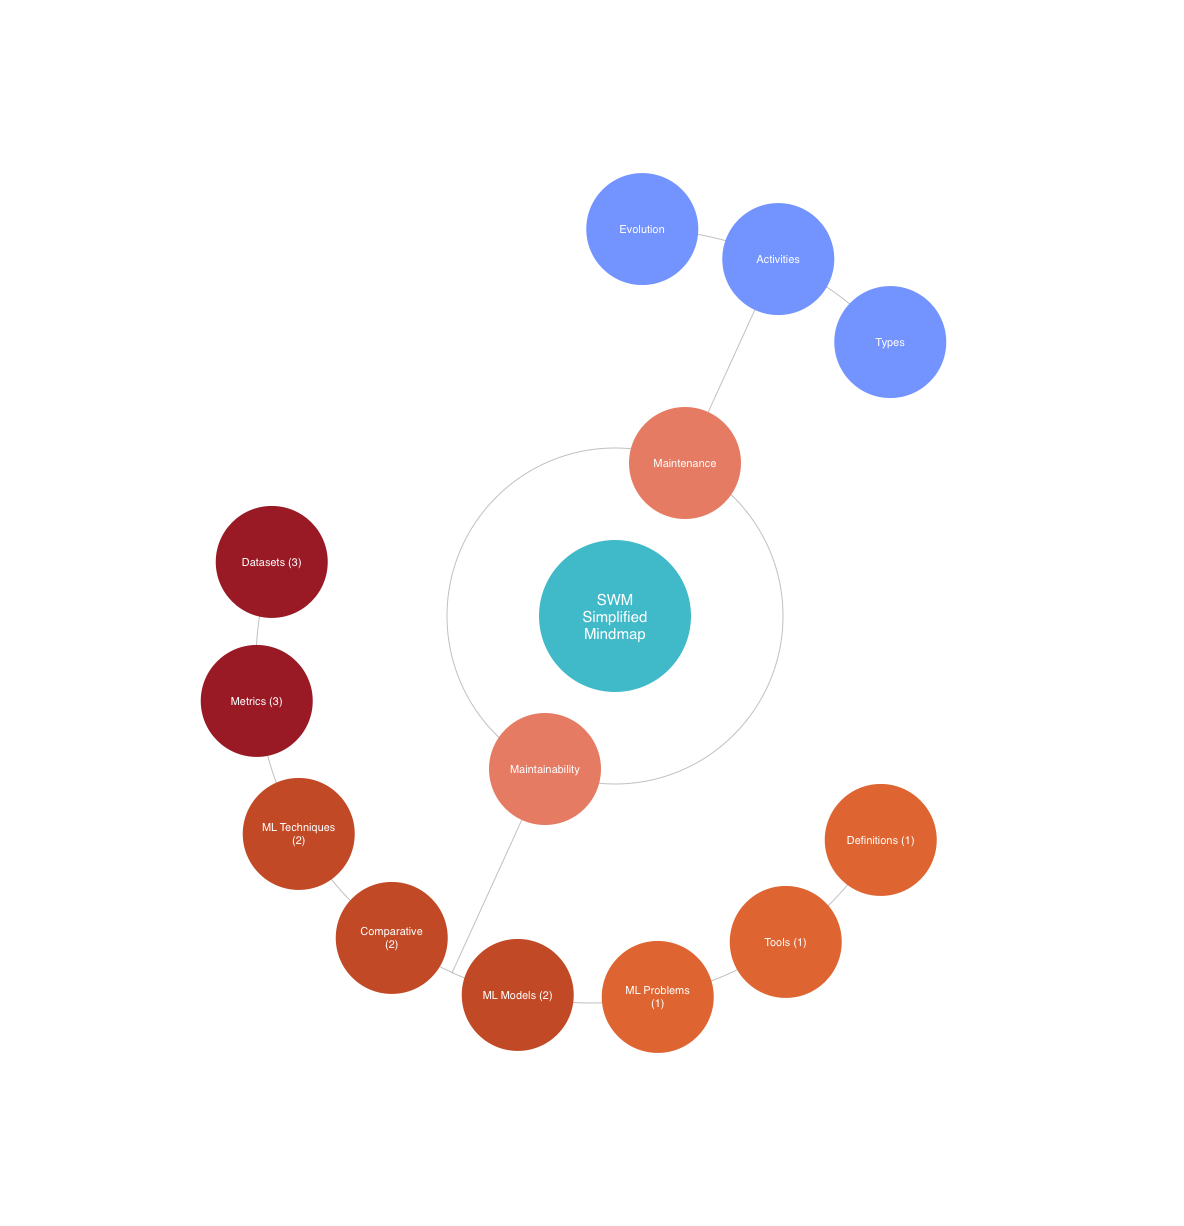
\includegraphics[width=8.5cm]{topics.png}
    \caption{Topics}
    \label{fig:topics}
\end{figure}

I have not included in the topic map the gaps that exist. Honestly, I need to read more. I can state that no one is writing about the importance of maintainability within vulnerable software. There is also no one speaking about the influence of maintenance as a metric to be centralized within software-based companies. I think these gaps can be addressed in the future. I will be adding those gaps in the future, as long as I am able to properly define and state those. I feel that adding something that might not be what I am looking for can distract me from my path.

\bibliographystyle{IEEEtran}
\bibliography{refs}

\end{document}